
%%%%%%%%%%%%%%%%%%%%%%%%
%
% $Autor: Keerti Belmane $
% $Datum: 2025-06-11 20:48:02Z $
% $Pfad: D:/BA_PROJECT/BA25-02-Time-Series/report/Contents/en/Monitoring.tex $
% $Version: 4621 $
%
% !TeX encoding = utf8
% !TeX root = Rename
%
%%%%%%%%%%%%%%%%%%%%%%%%



\chapter{Monitoring and Robustness}


\subsection{Idea}

The monitoring approach in our project ensures that the system remains stable, correct, and predictable whenever users upload new hurricane data. Since the application runs entirely on the user's local machine, no data is collected, stored, or transmitted externally. However, we've implemented several internal checks and automated test cases to ensure it.

\subsection{Alignment with PANKTI}

Our project’s monitoring approach aligns closely with the principles behind PANKTI, a production monitoring system proposed by \cite{Tiwari2021PANKTI}.



Similarly, \textbf{our project} runs entirely on the user’s local machine and monitors the system whenever new hurricane data is uploaded. Although we do not collect or transmit user data externally, \textbf{our project} implements internal checks and automated tests that:

\begin{itemize}
	\item Validate the uploaded data for correctness and consistency,
	\item Ensure that forecasting models (ARIMA/LSTM) behave as expected with new inputs,
	\item Detect anomalies or unusual prediction patterns to flag potential issues.
\end{itemize}

By continuously monitoring the system’s runtime behavior and running these automated checks, \textbf{our project} maintains stability and reliability, much like PANKTI’s goal of using live production data to strengthen software test suites. This alignment ensures that \textbf{our project} remains robust and trustworthy across varying real-world datasets.




The monitoring approach in our project ensures that the system remains stable, correct, and predictable whenever users upload new hurricane data. Since the application runs entirely on the user\textquotesingle{}s local machine, no data is collected, stored, or transmitted externally. However, we\textquotesingle ve implemented several internal checks and test cases to ensure:
\begin{itemize}
	\item The uploaded data is valid and clean,
	\item The forecasting models (ARIMA/LSTM) don\textquotesingle t crash or misbehave,
	\item The predictions are generated reliably.
\end{itemize}

\begin{center}
	\begin{tikzpicture}[
		node distance=1.5cm,
		every node/.style={
			rectangle, draw=black!70, fill=blue!10, rounded corners,
			minimum height=1cm, minimum width=6cm, align=center, font=\small
		},
		->, >=Stealth
		]
		
		\node (start) {System Input: User-Uploaded Data};
		\node (validate) [below=of start] {Check: Is the data valid and clean?};
		\node (model) [below=of validate] {Run ARIMA/LSTM Models (No crash)};
		\node (predict) [below=of model] {Generate Forecasts Reliably};
		\node (done) [below=of predict, draw=green!50!black, fill=green!20] {Output: Trusted Predictions};
		
		\draw (start) -- (validate);
		\draw (validate) -- (model);
		\draw (model) -- (predict);
		\draw (predict) -- (done);
		
	\end{tikzpicture}
\end{center}


We rely on unit and integration test cases to validate individual components like data loading, preprocessing, model execution, and the full pipeline. These checks make the system robust before it ever reaches the end-user. The system does \textbf{not} update itself automatically. Models are pre-trained and delivered with the tool.

\subsection{Monitoring Plan}
We test different aspects of the pipeline to ensure the hurricane prediction system works reliably:
\begin{itemize}
	\item Upload handling --- what happens if no file is uploaded?
	\item CSV validation --- columns, formats, types.
	\item Value checks --- wind speed should be numeric, dates convertible to datetime.
	\item Model execution --- ARIMA and LSTM should train, predict, and save properly.
	\item Edge cases --- what happens with very short datasets?
	\item End-to-end runs --- full forecasting without crash.
	\item Data cleaning --- missing values handled via interpolation.
\end{itemize}

\subsection{Getting New Data}
Users are expected to upload their own \texttt{.csv} files (e.g., hurricane wind speed and dates). The system does not provide or auto-load any example/demo data.

If \textbf{no file is uploaded}, the pipeline does \textbf{not} execute. Instead, it gracefully warns the user to upload a valid dataset. This design keeps the system lightweight and fully offline.

\subsection*{Data Updating in the ML Pipeline}
\begin{itemize}
	\item \textbf{Upload:} Users manually upload new storm data.
	\item \textbf{Forecasting:} Predictions are made using the pre-trained ARIMA or LSTM models.
	\item \textbf{Retraining:} If users wish to retrain models with new data, they can run the provided \texttt{developer.py} script. This is optional and manual.
\end{itemize}

\subsection{Evaluation Checks}
\begin{center}
	\renewcommand{\arraystretch}{1.1}
	\begin{tabular}{|c|p{4cm}|p{3.2cm}|p{4cm}|c|}
		\hline
		\textbf{Test ID} & \textbf{What It Checks} & \textbf{Input} & \textbf{Expected Output} & \textbf{Status} \\
		\hline
		TC01 & Upload missing & No file uploaded & App does not crash; shows prompt & \checkmark PASSED \\
		TC02 & File format & CSV file & DataFrame with correct format & \checkmark PASSED \\
		TC03 & Wind speed numeric & Sample data & All values numeric & \checkmark PASSED \\
		TC04 & Date format & Date strings & Converted to datetime & \checkmark PASSED \\
		TC05 & ARIMA training & Clean time series & Model trains correctly & \checkmark PASSED \\
		TC06 & ARIMA with short data & Few rows & Error/warning raised & \checkmark PASSED \\
		TC08 & Full pipeline & Real data & Forecast created & \checkmark PASSED \\
		TC10 & Missing values & NaNs in CSV & Filled via interpolation & \checkmark PASSED \\
		\hline
	\end{tabular}
\end{center}

\begin{figure}[H]
	\centering
	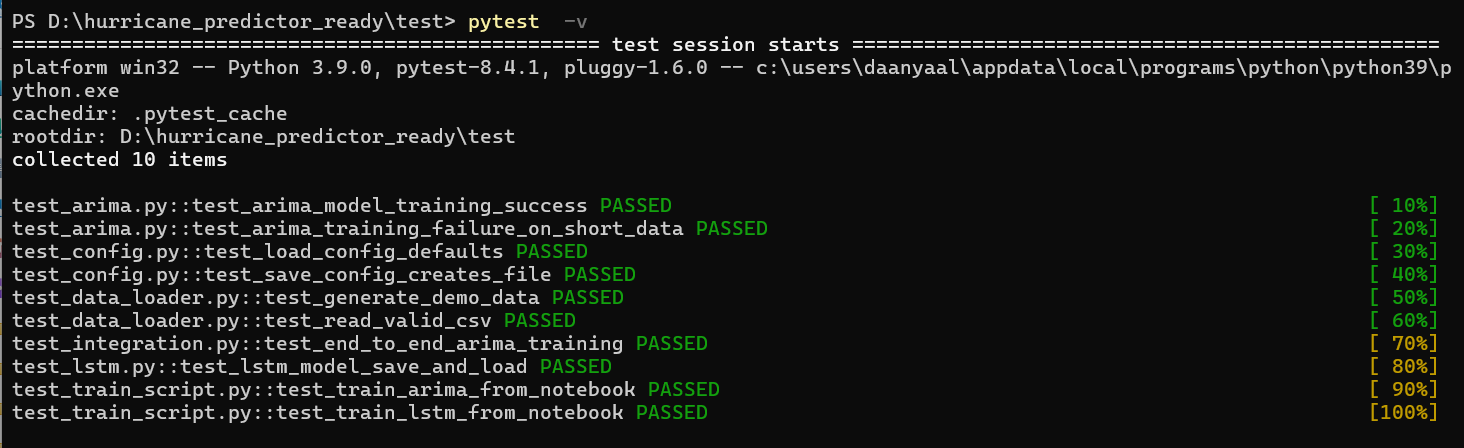
\includegraphics[width=1.2\textwidth, height=0.9\textheight, keepaspectratio]{../../BA25-02-Time-Series/report/Images/testoutput.png}
	\caption[Visualization of Test Output Results]{
		Visualization of the test output generated during the system validation phase.
	}
	\label{fig:outputs}
\end{figure}

\subsection{Code: Functions}

\begin{lstlisting}[language=Python,caption={Test LSTM File }, label={LSTMTesting}]
import numpy as np
from sklearn.preprocessing import MinMaxScaler
from tensorflow.keras.models import Sequential
from tensorflow.keras.layers import LSTM, Dense
from model_utils import save_lstm_model, load_lstm_model  # adjust if needed

def test_lstm_model_save_and_load(tmp_path):
	print("Running test_lstm_model_save_and_load")
	model = Sequential([
	LSTM(10, input_shape=(10, 1)),
	Dense(1)
	])
	model.compile(optimizer='adam', loss='mse')
	
	scaler = MinMaxScaler()
	dummy_data = np.random.rand(100, 1)
	scaler.fit(dummy_data)
	
	model_path = tmp_path / "test_lstm_model.h5"
	scaler_path = tmp_path / "test_scaler.pkl"
	save_lstm_model(model, scaler, str(model_path), str(scaler_path))
	
	loaded_model, loaded_scaler = load_lstm_model(str(model_path), str(scaler_path))
	assert loaded_model is not None
	assert loaded_scaler is not None
	print("Finished test_lstm_model_save_and_load")

\end{lstlisting}

\subsubsection{Functions used}
\begin{itemize}
	\item \textbf{test\_lstm\_model\_save\_and\_load}: This function checks (tests) whether a model and its scaler can be saved and loaded correctly. It combines steps like building a model, scaling some data, saving, and loading back.
	\item \textbf{save\_lstm\_model}: Saves the model and scaler to disk.
	\item \textbf{load\_lstm\_model}: Loads the model and scaler back from disk.
	\item \textbf{print}: Shows progress messages in the console.
	\item \textbf{assert}: Checks that what was loaded is not None (to catch errors).
\end{itemize}

\subsubsection{Why are they being used?}
\begin{itemize}
	\item \textbf{To organize code}:\\
	The main test logic is inside a function (test\_lstm\_model\_save\_and\_load).
	This makes it reusable, easier to test, and more readable.
	\item \textbf{To avoid repetition}:\\
	If we want to check saving/loading with different paths or models,
	we just call the function again with different arguments.
	\item \textbf{For modularity}:\\
	We can use save\_lstm\_model and load\_lstm\_model elsewhere in our code with any LSTM model and scaler.
	\item \textbf{For clarity}:\\
	Each function does one job, making the steps in our workflow clearer and code easier to maintain.
	\item \textbf{For testing}:\\
	Having tests in functions is a standard practice for checking if everything is working as expected
\end{itemize}

\newpage
\subsection{Code: Test}

\begin{lstlisting}[language=Python,caption={Integration testing}, label={integrationTest}]
	import numpy as np
	import pandas as pd
	from model_utils import load_config, save_config, train_arima_model  # Adjust import path if needed
	
	def test_end_to_end_arima_training(tmp_path):
		print("Starting end-to-end ARIMA training test")
		config_path = tmp_path / "config.json"
		config = load_config(config_path)
		config["arima"]["p"] = 1
		config["arima"]["d"] = 1
		config["arima"]["q"] = 1
		save_config(config, config_path, username="test_runner")
		
		df = pd.DataFrame({
			"date": pd.date_range("2022-01-01", periods=50),
			"wind_speed": np.random.normal(60, 10, 50)
		})
		
		model = train_arima_model(df["wind_speed"], (1, 1, 1))
		assert model is not None
		print("Completed end-to-end ARIMA training test")
	
	
\end{lstlisting}

We carried out integration testing. In integration testing we are testing how several parts of our code (modules, functions) work together. Here, we are checking not just one function but the whole flow: loading configs, saving them, making random data, and training and returning a model.

\renewcommand{\arraystretch}{1.4} % makes it look nicer

\begin{table}[H]
	\centering
	\caption{Explanation of Integration Testing Steps}
	\begin{tabularx}{\textwidth}{|l|X|X|}
		\hline
		\textbf{Line/Function} & \textbf{What it does} & \textbf{Why it’s used} \\
		\hline
		\texttt{def test\_end\_to\_end\_arima\_training} & Defines a test procedure (function) & Easy to run and reuse the test as a single unit \\
		\hline
		\texttt{print(...)} & Outputs info about the test’s progress & Easier to debug \\
		\hline
		\texttt{config = load\_config(config\_path)} & Loads configuration file & Tests that config loading works \\
		\hline
		Update \texttt{config["arima"]["p/d/q"]} & Changes ARIMA hyperparameters & Checks if we can change config and pass new parameters \\
		\hline
		\texttt{save\_config(...)} & Saves the config back & Ensures saving config works as expected \\
		\hline
		\texttt{df = pd.DataFrame(\{....\})} & Makes a sample dataset for testing & Provides test input for the model \\
		\hline
		\texttt{model = train\_arima\_model(...)} & Trains the ARIMA model & Integrates several components: data and config \\
		\hline
		\texttt{assert model is not None} & Checks that model is returned & Validates final output: if fails, test "breaks" \\
		\hline
		\texttt{print(...)} & Marks test completion & For clarity/feedback \\
		\hline
	\end{tabularx}
\end{table}

\subsection{Privacy}
\begin{itemize}
	\item All data stays on the user\textquotesingle s local machine.
	\item No files are uploaded, stored, or accessed remotely.
	\item Users control inputs, models, and outputs.
	\item No personally identifiable information (PII) is handled.
	\item Ethical AI principles followed:
	\begin{itemize}
		\item Model explainability
		\item Offline operation
		\item Full control by user
	\end{itemize}
\end{itemize}

\subsection{Robustness Features}
\begin{itemize}
	\item \textbf{No Upload \ensuremath{\Rightarrow} No Crash:} If no file is uploaded, the system shows a prompt. \textit{(TC01)}
	\item \textbf{Bad Input Check:} Verifies wind speed type, date format, missing values. \textit{(TC03, TC04, TC10)}
	\item \textbf{Handles Tiny Data:} ARIMA raises clear error if data is insufficient. \textit{(TC06)}
	\item \textbf{End-to-End Validation:} The pipeline runs reliably. \textit{(TC08)}
	\item \textbf{Model Save/Reload:} LSTM and scalers work across sessions. \textit{(TC07)}
	\item \textbf{Offline First:} No server/API reliance.
\end{itemize}

\subsection{End-to-End User Process}
\begin{enumerate}
	\item \textbf{Upload .csv File:} Required columns: wind speed, date \hfill (\textit{TC01, TC02})
	\item \textbf{Data Cleaning:} Numeric check, date parsing, interpolation \hfill (\textit{TC03, TC04, TC10})
	\item \textbf{Prediction:} Models forecast automatically \hfill (\textit{TC05, TC08})
	\item \textbf{Results Display:} Forecast is shown and downloadable
	\item \textbf{Optional Retraining:} \texttt{developer.py} enables training with new data \hfill (\textit{TC06, TC09})
	\item \textbf{Repeat:} Upload and forecast again anytime
\end{enumerate}
